\documentclass[12pt,a4paper]{article}
\usepackage[utf8]{inputenc}
\usepackage[T1]{fontenc}
\usepackage{amsmath, amssymb, amsthm}
\usepackage{geometry}

% Definir entornos de teoremas
\newtheorem{theorem}{Teorema}
\newtheorem{lemma}{Lema}
\newtheorem{corollary}{Corolario}
\newtheorem{proposition}{Proposición}
\usepackage{tikz}
\usetikzlibrary{automata,positioning}
\geometry{margin=1in}
\usepackage{enumitem}
\usepackage[framemethod=tikz]{mdframed}

% Eliminar sangría de párrafos
\setlength{\parindent}{0pt}

% Macro para definiciones
\newmdenv[
    backgroundcolor=blue!5,
    linecolor=blue!40,
    linewidth=1.5pt,
    roundcorner=5pt,
    innertopmargin=8pt,
    innerbottommargin=8pt,
    innerleftmargin=10pt,
    innerrightmargin=10pt,
    leftmargin=0pt,
    rightmargin=0pt
]{definicionbox}

\newcommand{\definicion}[1]{%
\begin{definicionbox}
\textbf{Definición}: #1
\end{definicionbox}
}

% Macro para teoremas
\newmdenv[
    backgroundcolor=green!5,
    linecolor=green!50,
    linewidth=1.5pt,
    roundcorner=5pt,
    innertopmargin=8pt,
    innerbottommargin=8pt,
    innerleftmargin=10pt,
    innerrightmargin=10pt,
    leftmargin=0pt,
    rightmargin=0pt
]{teoremabox}

\newcommand{\teorema}[1]{%
\begin{teoremabox}
\textbf{Teorema}: #1
\end{teoremabox}
}

\title{Apuntes de Procesos Estocásticos}
\author{}
\date{}

\begin{document}
\maketitle

% ===================== Datos generales =====================
\section{Datos del curso}
\begin{itemize}
    \item \textbf{Profesor:} Nicolás Moreno
    \item \textbf{Correo:} \texttt{namorenor@eafit.edu.co}
    \item \textbf{Oficina:} 19-604
    \item \textbf{Horario de atención:} Jueves 10:00 a 13:00
\end{itemize}

\subsection*{Contenido}
\begin{enumerate}
    \item Cadenas de Markov en tiempo discreto.
    \item Procesos de Poisson.
    \item Cadenas de Markov en tiempo continuo.
    \item Teoría de filas.
    \item Martingalas.
\end{enumerate}

\subsection*{Parciales}
\begin{itemize}
    \item Parcial 1: Semana 5 (21 de agosto) \hfill (25\%)
    \item Parcial 2: Semana 11 (22 de septiembre) \hfill (25\%)
    \item Parcial 3: Semana 17 (10 de noviembre) \hfill (25\%)
\end{itemize}

\subsection*{Talleres de seguimiento}
\begin{itemize}
    \item Taller: Semana 5 \hfill (5\%)
    \item Taller: Semana 11 \hfill (5\%)
\end{itemize}

\subsection*{Bibliografía}
\begin{itemize}
    \item Durrett, R. \textit{Essentials of Stochastic Processes}.
    \item Ross, S. \textit{Stochastic Processes}.
\end{itemize}

% ===================== Procesos estocásticos =====================
\section{¿Qué es un proceso estocástico?}
\definicion{Un \textbf{proceso estocástico} es una colección de variables aleatorias
\begin{equation*}
\{X_t\}_{t\in T},
\end{equation*}
donde $T$ puede ser finito, numerable o no numerable.
\begin{itemize}
    \item Si $T$ es finito o numerable, el proceso es \textbf{discreto}.
    \item Si $T$ es no numerable, el proceso es \textbf{continuo}.
\end{itemize}
El conjunto de posibles valores de $X_t$ se denota por $S$ y se llama \textbf{espacio de estados}. Al igual que $T$, $S$ puede ser discreto o continuo.}

\textbf{Ejemplo}: Artículos defectuosos
\begin{enumerate}
    \item Número de artículos defectuosos producidos por una máquina cada hora:
    \begin{equation*}
    T:\ \text{discreto}, \qquad S:\ \text{discreto}.
    \end{equation*}
    \item Nivel de agua en una represa:
    \begin{equation*}
    T:\ \text{continuo}, \qquad S:\ \text{continuo}.
    \end{equation*}
    \item Número de clientes haciendo fila:
    \begin{equation*}
    T:\ \text{continuo}, \qquad S:\ \text{discreto}.
    \end{equation*}
    \item Tiempos entre llegadas de clientes
    \begin{align*}
        X_1 &: \text{tiempo hasta la primera llegada},\\
        X_2 &: \text{tiempo entre las llegadas 1 y 2},\\
        X_3 &: \text{tiempo entre las llegadas 2 y 3},\ \ldots
    \end{align*}
    \begin{equation*}
    T:\ \text{discreto}, \qquad S:\ \text{continuo}.
    \end{equation*}
\end{enumerate}

\definicion{Un proceso estocástico puede verse como una función
\begin{equation*}
X:\ \Omega \times T \longrightarrow \mathbb{R},\qquad (\omega,t)\mapsto X(\omega,t).
\end{equation*}
\begin{itemize}
    \item Si $t$ es fijo, $\omega \mapsto X(\omega,t)$ es una variable aleatoria.
    \item Si $\omega$ es fijo, $t \mapsto X(\omega,t)$ es una trayectoria.
\end{itemize}}

\textbf{1. Espacio de probabilidad:}
\begin{itemize}
    \item $\Omega$ es el conjunto de todos los posibles resultados (espacio muestral).
    \item Cada elemento $\omega \in \Omega$ representa un \textbf{experimento completo} o un \textbf{escenario particular}.
\end{itemize}

\textbf{2. Proceso estocástico como función:}

Formalmente, un proceso estocástico es una función de dos variables:
\begin{equation*}
X : \Omega \times T \to \mathbb{R}
\end{equation*}

donde:
\begin{itemize}
    \item $\Omega$ captura la aleatoriedad (cada $\omega$ es un "universo" posible).
    \item $T$ es el conjunto de tiempos (índice temporal).
    \item El valor $X(\omega, t)$ es el \textbf{estado} que el proceso tiene en el tiempo $t$ en el escenario $\omega$.
\end{itemize}

\textbf{3. Interpretación práctica:}
\begin{itemize}
    \item Fija un $\omega$: obtienes una \textbf{trayectoria} o \textbf{realización} del proceso en todo $t$.
    \item Fija un $t$: obtienes una \textbf{variable aleatoria} $X_t(\omega) = X(\omega, t)$ que describe el estado en ese instante, pero depende del azar.
\end{itemize}

\textbf{Ejemplo}: Clientes en fila
\begin{center}
\begin{tikzpicture}[scale=1]
    \draw[->] (0,0) -- (5.2,0) node[right] {$t$};
    \draw[->] (0,0) -- (0,3.6) node[above] {Número de clientes};
    \draw[thick] (0,1) -- (1,1);
    \draw[thick] (1,2) -- (3,2);
    \draw[thick] (3,3) -- (4,3);
    \fill (1,1) circle (2pt);
    \fill (3,2) circle (2pt);
    \draw (1,2) circle (2pt);
    \draw (3,3) circle (2pt);
    \node at (0,-0.3) {$t_0$};
    \node at (1,-0.3) {$t_1$};
    \node at (3,-0.3) {$t_2$};
    \node at (4,-0.3) {$t_3$};
\end{tikzpicture}
\end{center}

% ===================== Cadenas de Markov =====================
\section{Cadenas de Markov en tiempo discreto}
\definicion{Un proceso $\{X_n\}_{n\ge 0}$ con espacio de estados $S$ es una \textbf{cadena de Markov} si para todo
$i,j,i_0,\ldots,i_{n-1}\in S$ y $n=0,1,2,\ldots$,
\begin{equation*}
P(X_{n+1}=j \mid X_n=i, X_{n-1}=i_{n-1},\ldots,X_0=i_0)
= P(X_{n+1}=j \mid X_n=i).
\end{equation*}}

\subsection*{Probabilidad de transición}
La probabilidad
\begin{equation*}
P(X_{n+1}=j \mid X_n=i)
\end{equation*}
se llama \textbf{probabilidad de transición} del estado $i$ al estado $j$ en un paso.

\subsection*{Cadena homogénea y matriz de transición}
Si $P(X_{n+1}=j \mid X_n=i)$ no depende de $n$, la cadena es \textbf{homogénea} y se escribe
\begin{equation*}
P(X_{n+1}=j \mid X_n=i)=P_{ij}.
\end{equation*}
Las probabilidades $P_{ij}$ se organizan en la \textbf{matriz de transición} $P=(P_{ij})$, cuyas filas verifican
$\sum_j P_{ij}=1$ y $P_{ij}\ge 0$.

\textbf{Ejemplo}: Matriz $2\times 2$ y grafo
\begin{equation*}
P=\begin{pmatrix}
\alpha & 1-\alpha\\
\beta & 1-\beta
\end{pmatrix}
\end{equation*}
\begin{center}
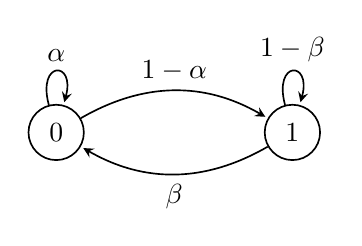
\begin{tikzpicture}[->,>=stealth,shorten >=1pt,auto,node distance=3cm,semithick]
\tikzstyle{every state}=[fill=white,draw=black,text=black,minimum size=20pt]
\node[state] (A) {$0$};
\node[state] (B) [right of=A] {$1$};
\path
(A) edge[loop above] node{$\alpha$} (A)
(A) edge[bend left] node{$1-\alpha$} (B)
(B) edge[bend left] node{$\beta$} (A)
(B) edge[loop above] node{$1-\beta$} (B);
\end{tikzpicture}
\end{center}

\textbf{Ejemplo (modelo de lluvia)}:
Estados $0=$lluvia, $1=$no lluvia. Con parámetros $\alpha,\beta$:
\begin{equation*}
P(X_{n+1}=0 \mid X_n=0)=\alpha, \qquad
P(X_{n+1}=0 \mid X_n=1)=\beta.
\end{equation*}

\textbf{Ejemplo (juego de apuestas)}: En cada juego se gana $1$ con probabilidad $0.6$ y se pierde $1$ con probabilidad $0.4$.
El jugador se retira al llegar a $0$ o $4$. Sea $X_n$ la cantidad de dinero al tiempo $n$.
\begin{equation*}
P=
\begin{pmatrix}
1 & 0 & 0 & 0 & 0\\
0.4 & 0 & 0.6 & 0 & 0\\
0 & 0.4 & 0 & 0.6 & 0\\
0 & 0 & 0.4 & 0 & 0.6\\
0 & 0 & 0 & 0 & 1
\end{pmatrix}
\end{equation*}
\begin{center}
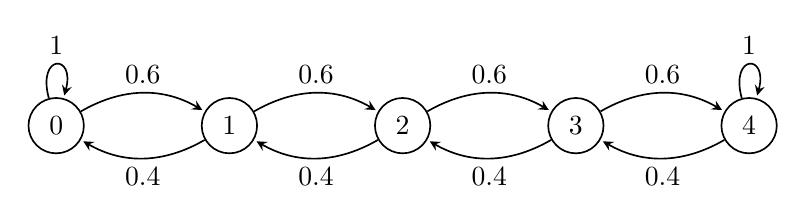
\begin{tikzpicture}[->,>=stealth,shorten >=1pt,auto,node distance=2.2cm,semithick]
\tikzstyle{every state}=[fill=white,draw=black,text=black,minimum size=20pt]
\node[state] (A) {$0$};
\node[state] (B) [right of=A] {$1$};
\node[state] (C) [right of=B] {$2$};
\node[state] (D) [right of=C] {$3$};
\node[state] (E) [right of=D] {$4$};
\path
(A) edge[loop above] node{$1$} (A)
(E) edge[loop above] node{$1$} (E)
(A) edge[bend left] node{$0.6$} (B)
(B) edge[bend left] node{$0.4$} (A)
(B) edge[bend left] node{$0.6$} (C)
(C) edge[bend left] node{$0.4$} (B)
(C) edge[bend left] node{$0.6$} (D)
(D) edge[bend left] node{$0.4$} (C)
(D) edge[bend left] node{$0.6$} (E)
(E) edge[bend left] node{$0.4$} (D);
\end{tikzpicture}
\end{center}

\textbf{Ejemplo (paseo aleatorio)}: Considere un proceso $\{X_n\}_{n\ge 0}$ con espacio de estados $S=\mathbb{Z}$ y sus probabilidades de transición están dadas por:

\begin{align*}
    P(i,i+1) &= p \\
    P(i,i-1) &= q
\end{align*}

De forma más general:

\begin{equation*}
P(i,j)=
\begin{cases}
p, \text{ si } j=i+1,\\
q, \text{ si } j=i-1,\\
r, \text{ si } j = i
\end{cases}
\qquad p + q + r = 1.
\end{equation*}
\begin{center}
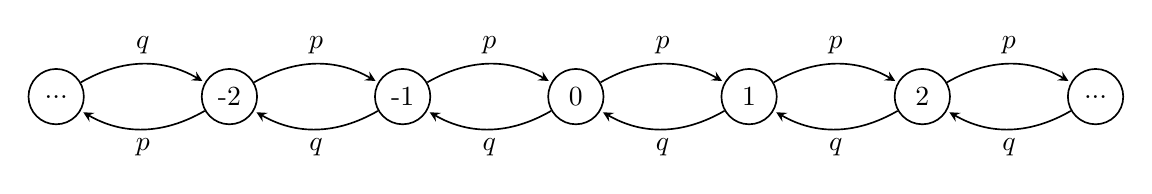
\begin{tikzpicture}[->,>=stealth,shorten >=1pt,auto,node distance=2.2cm,semithick]
\tikzstyle{every state}=[fill=white,draw=black,text=black,minimum size=20pt]

\node[state] (Z) {...};
\node[state] (A) [right of=Z] {-2};
\node[state] (B) [right of=A] {-1};
\node[state] (C) [right of=B] {0};
\node[state] (D) [right of=C] {1};
\node[state] (E) [right of=D] {2};
\node[state] (F) [right of=E] {...};
\path
(Z) edge[bend left] node{$q$} (A)
(A) edge[bend left] node{$p$} (Z)
(A) edge[bend left] node{$p$} (B)
(B) edge[bend left] node{$q$} (A)
(B) edge[bend left] node{$p$} (C)
(C) edge[bend left] node{$q$} (B)
(C) edge[bend left] node{$p$} (D)
(D) edge[bend left] node{$q$} (C)
(D) edge[bend left] node{$p$} (E)
(E) edge[bend left] node{$q$} (D)
(E) edge[bend left] node{$p$} (F)
(F) edge[bend left] node{$q$} (E);
\end{tikzpicture}
\end{center}

% ===================== Ramificación =====================
\textbf{Ejemplo (ramificación)}: Supóngase que un organismo tiene $j$ hijos con probabilidad $\alpha_j$:
\begin{equation*}
    P(Z=j)=\alpha_j
\end{equation*}

donde $Z$ es el número de hijos de un individuo.

\begin{itemize}
    \item $X_0$: número de individuos en la generación 0.
    \item $X_1$: número de individuos en la generación 1.
    \item $X_2$: número de individuos en la generación 2, etc.
\end{itemize}

\begin{equation*}
P(X_{n+1}=j \mid X_n=i)=
\begin{cases}
0, & i=0,\ j>0,\\
1, & i=0,\ j=0,\\
P\!\left(\sum_{k=1}^{i} Z_k=j\right), & i>0,\ j\ge 0,
\end{cases}
\end{equation*}
donde $Z_k$ son independientes con la misma ley que $Z$.

\begin{center}
\begin{tikzpicture}[scale=1]
% Nodo central X_0 alineado con tiempo 0
\node[circle, fill=black, minimum size=4pt, inner sep=0pt] (X0) at (0,2) {}; % Nodo X_0
\node[left] at (-0.3,2) {$X_0$};

% Tres puntos alineados con tiempo 1
\node[circle, fill=black, minimum size=4pt, inner sep=0pt] (Z1) at (1.5,2.8) {}; % Nodo Z_1
\node[left] at (1.2,2.8) {$Z_1$};
\node[circle, fill=black, minimum size=4pt, inner sep=0pt] (Z2) at (1.5,2) {}; % Nodo Z_2
\node[left] at (1.2,2) {$Z_2$};
\node[circle, fill=black, minimum size=4pt, inner sep=0pt] (Z3) at (1.5,1.2) {}; % Nodo Z_3
\node[left] at (1.2,1.2) {$Z_3$};

\draw[->] (X0) -- (Z1);
\draw[->] (X0) -- (Z2);
\draw[->] (X0) -- (Z3);

% Cinco puntos alineados con tiempo 2
\node[circle, fill=black, minimum size=4pt, inner sep=0pt] (Q1)at (3,3.8) {};
\node[circle, fill=black, minimum size=4pt, inner sep=0pt] (Q2) at (3,3) {};
\node[circle, fill=black, minimum size=4pt, inner sep=0pt] (Q3) at (3,1.8) {};
\node[circle, fill=black, minimum size=4pt, inner sep=0pt] (Q4) at (3,1.0) {};
\node[circle, fill=black, minimum size=4pt, inner sep=0pt] (Q5) at (3,0.2) {};

\draw[->] (Z1) -- (Q1);
\draw[->] (Z1) -- (Q2);

\draw[->] (Z3) -- (Q3);
\draw[->] (Z3) -- (Q4);
\draw[->] (Z3) -- (Q5);

% Línea horizontal de tiempo
\draw[thick] (-1,-1) -- (6,-1);
\node[below] at (0,-1) {0};
\node[below] at (1.5,-1) {1};
\node[below] at (3,-1) {2};
\node[below] at (4,-1) {...};
\node[below] at (5.5,-1) {$n$};

\end{tikzpicture}
\end{center}

\textbf{Ejemplo (urna de Ehrenfest)}: Suponga que hay $N$ bolas numeradas de $1$ a $N$ y distribuidas en 2 urnas.  
En el tiempo $n$ se selecciona al azar una bola del conjunto $\{1, 2, \ldots, N\}$.

\begin{itemize}
    \item Si la bola corresponde a una de la urna 1, se pasa a la urna 2.
    \item Si la bola corresponde a una de la urna 2, se pasa a la urna 1.
\end{itemize}

Sea $X_n$ el número de bolas en la urna 1 en el tiempo $n$.  
El diagrama de estados es:

\begin{center}
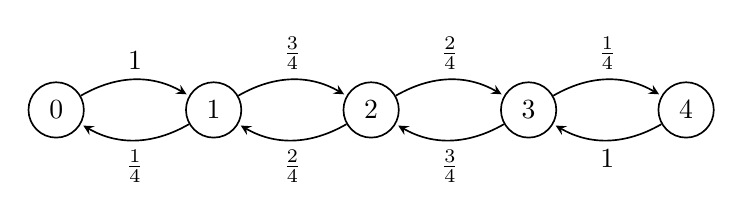
\begin{tikzpicture}[scale=1,->,>=stealth,shorten >=1pt,auto,node distance=2cm,semithick]
\tikzstyle{every state}=[fill=white,draw=black,text=black,minimum size=20pt]
\node[state] (A) {0};
\node[state] (B) [right of=A] {1};
\node[state] (C) [right of=B] {2};
\node[state] (D) [right of=C] {3};
\node[state] (E) [right of=D] {4};

\path
(A) edge[bend left] node{$1$} (B)
(B) edge[bend left] node{$\frac{1}{4}$} (A)
(B) edge[bend left] node{$\frac{3}{4}$} (C)
(C) edge[bend left] node{$\frac{2}{4}$} (B)
(C) edge[bend left] node{$\frac{2}{4}$} (D)
(D) edge[bend left] node{$\frac{3}{4}$} (C)
(D) edge[bend left] node{$\frac{1}{4}$} (E)
(E) edge[bend left] node{$1$} (D);
\end{tikzpicture}
\end{center}

La matriz de transición $P$ para $N$ bolas es:

\begin{equation*}
P =
\begin{pmatrix}
0 & 1 & 0 & 0 & \cdots & 0 & 0 \\
\frac{1}{N} & 0 & \frac{N-1}{N} & 0 & \cdots & 0 & 0 \\
0 & \frac{2}{N} & 0 & \frac{N-2}{N} & \cdots & 0 & 0 \\
0 & 0 & \frac{3}{N} & 0 & \cdots & 0 & 0 \\
\vdots & \vdots & \vdots & \vdots & \ddots & \vdots & \vdots \\
0 & 0 & 0 & 0 & \cdots & 0 & 1 \\
0 & 0 & 0 & 0 & \cdots & \frac{1}{N} & 0
\end{pmatrix}
\end{equation*}

donde:
\begin{itemize}
    \item $X_0$: número de bolas en la urna 1 en el tiempo inicial.
    \item $X_1$: número de bolas en la urna 1 en el siguiente paso.
\end{itemize}

Las probabilidades de transición son:
\begin{equation*}
P(X_{n+1} = j \mid X_n = i) =
\begin{cases}
\frac{N-i}{N}, & \text{si } j = i+1 \text{ (se transfiere de urna 2 a urna 1)},\\
\frac{i}{N}, & \text{si } j = i-1 \text{ (se transfiere de urna 1 a urna 2)},\\
0, & \text{en cualquier otro caso}.
\end{cases}
\end{equation*}

\textbf{Problema:} Sea $X_n$ el clima en el día $n$. Suponga que un modelo para este proceso es una 
\textbf{cadena de Markov} con matriz de transición dada por

\begin{equation*}
P =
\begin{pmatrix}
0.4 & 0.6 & 0.0 \\
0.2 & 0.5 & 0.3 \\
0.1 & 0.7 & 0.2
\end{pmatrix}
\end{equation*}

donde los estados son:
\begin{equation*}
1 = \text{Lluvia}, \quad
2 = \text{Nublado}, \quad
3 = \text{Sol}.
\end{equation*}

Hoy es lunes y está nublado. ¿Cuál es la probabilidad de que el martes esté soleado 
y el miércoles esté lloviendo?

Un proceso estocástico $\{X_n\}$ cumple que:
\begin{equation*}
P(X_n = j \mid X_{n-1} = i, X_{n-2} = i_{n-2}, \ldots, X_0 = i_0) 
= P(X_n = j \mid X_{n-1} = i) = P_{ij}.
\end{equation*}

\textbf{Solución}:

Se busca:
\begin{equation*}
P(X_2 = 1, \, X_1 = 3 \mid X_0 = 2).
\end{equation*}

Por la propiedad de Markov:
\begin{equation*}
P(X_2 = 1, \, X_1 = 3 \mid X_0 = 2) = P(2,3) \cdot P(3,1).
\end{equation*}

Usando la matriz de transición:
\begin{equation*}
P(2,3) = 0.3, \quad P(3,1) = 0.1,
\end{equation*}

entonces:
\begin{equation*}
P(X_2 = 1, \, X_1 = 3 \mid X_0 = 2) = 0.3 \times 0.1 = 0.03.
\end{equation*}

\tikzset{state/.style={circle,draw,minimum size=22pt,inner sep=0pt}}

\begin{center}
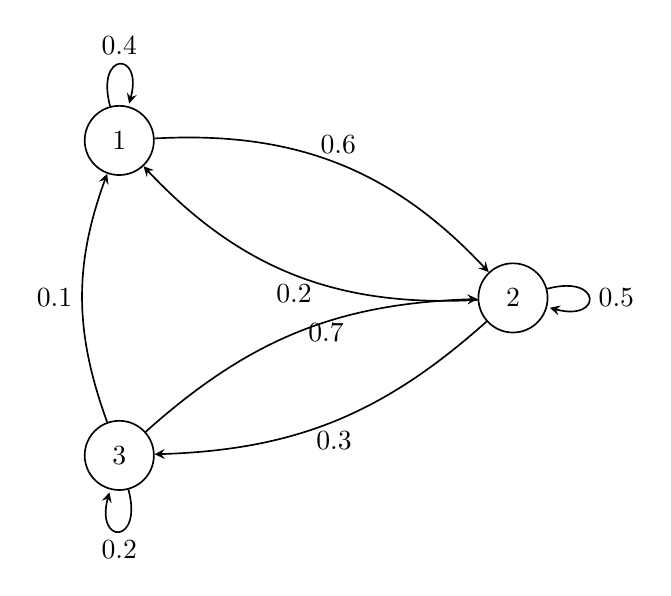
\begin{tikzpicture}[->,>=stealth,auto,semithick]
  % Nodos (estados 1,2,3)
  \node[state] (s1) at (0,2.0) {1};
  \node[state] (s2) at (5,0)   {2};
  \node[state] (s3) at (0,-2.0){3};

  % Bucles
  \path (s1) edge[loop above] node{$0.4$} (s1);
  \path (s2) edge[loop right] node{$0.5$} (s2);
  \path (s3) edge[loop below] node{$0.2$} (s3);

  % Transiciones 1 <-> 2
  \path (s1) edge[bend left=25] node[above] {$0.6$} (s2);
  \path (s2) edge[bend left=25] node[below] {$0.2$} (s1);

  % Transiciones 2 <-> 3
  \path (s2) edge[bend left=20] node[below] {$0.3$} (s3);
  \path (s3) edge[bend left=20] node[right] {$0.7$} (s2);

  % Transición 3 -> 1
  \path (s3) edge[bend left=20] node[left] {$0.1$} (s1);
  % No hay 1 -> 3 (probabilidad 0 en la matriz)
\end{tikzpicture}
\end{center}

\subsection*{Probabilidades de transición en $n$ pasos}

\definicion{Las probabilidades de transición en $n$ pasos del estado $i$ al estado $j$ se denotan por:
\begin{equation*}
p_{ij}^{(n)} = P(X_n = j \mid X_0 = i), \quad n \geq 0, \ i, j \in S.
\end{equation*}

En particular:
\begin{equation*}
p_{ij}^{(1)} = P_{ij}, \quad p_{ij}^{(0)} = \delta_{ij}
\end{equation*}
donde $\delta_{ij}$ es el delta de Kronecker. Se organiza en la matriz:
\begin{equation*}
P^{(n)} =
\begin{pmatrix}
p_{11}^{(n)} & p_{12}^{(n)} & p_{13}^{(n)} \\
p_{21}^{(n)} & p_{22}^{(n)} & p_{23}^{(n)} \\
p_{31}^{(n)} & p_{32}^{(n)} & p_{33}^{(n)}
\end{pmatrix}
\end{equation*}

}

\textbf{Propiedades}:
\begin{itemize}
    \item $P^{(0)} = I$ (matriz identidad).
    \item $P^{(1)} = P$ (matriz de transición de un paso).
\end{itemize}

\teorema{
\begin{equation*}
P^{(n)} = P^{(m)} \cdot P^{(n-m)}, \quad \text{en particular } P^{(n)} = P \cdot P \cdots P \ (\text{$n$ veces}) = P^n.
\end{equation*}}

\section*{Ecuaciones de Chapman--Kolmogorov}

Las \textbf{ecuaciones de Chapman--Kolmogorov} calculan las probabilidades de transición en múltiples pasos. Estas ecuaciones establecen que la probabilidad de transición del estado $i$ al estado $j$ en $n+m$ pasos puede descomponerse como la suma de todas las posibles transiciones intermedias a través de estados $k$ en el paso $n$.

\begin{center}
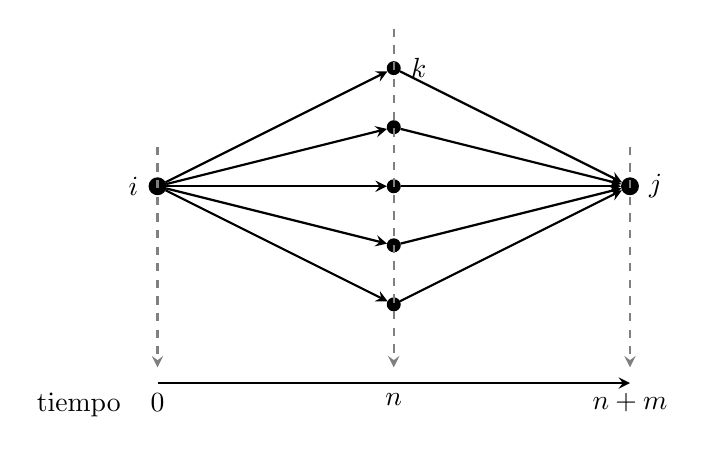
\begin{tikzpicture}[->, >=stealth, node distance=2cm, thick]

% Nodos principales
\node[circle, draw, fill=black, inner sep=2pt] (i) at (0,0) {};
\node[circle, draw, fill=black, inner sep=2pt] (j) at (6,0) {};

% Nodos intermedios k
\node[circle, draw, fill=black, inner sep=1.5pt] (k1) at (3,1.5) {};
\node[circle, draw, fill=black, inner sep=1.5pt] (k2) at (3,0.75) {};
\node[circle, draw, fill=black, inner sep=1.5pt] (k3) at (3,0) {};
\node[circle, draw, fill=black, inner sep=1.5pt] (k4) at (3,-0.75) {};
\node[circle, draw, fill=black, inner sep=1.5pt] (k5) at (3,-1.5) {};

% Etiquetas de estados
\node[left] at (i.west) {$i$};
\node[right] at (j.east) {$j$};
\node[right] at (k1.east) {$k$};

% Flechas rectas desde i hacia los k
\draw[->] (i) -- (k1);
\draw[->] (i) -- (k2);
\draw[->] (i) -- (k3);
\draw[->] (i) -- (k4);
\draw[->] (i) -- (k5);

% Flechas rectas desde los k hacia j
\draw[->] (k1) -- (j);
\draw[->] (k2) -- (j);
\draw[->] (k3) -- (j);
\draw[->] (k4) -- (j);
\draw[->] (k5) -- (j);

% Línea de tiempo
\draw[thick] (0,-2.5) -- (6,-2.5);
\node[below] at (0,-2.5) {$0$};
\node[below] at (3,-2.5) {$n$};
\node[below] at (6,-2.5) {$n+m$};
\node[below] at (-1,-2.5) {tiempo};

% Líneas verticales punteadas
\draw[dashed, gray] (0,0.5) -- (0,-2.3);
\draw[dashed, gray] (3,2) -- (3,-2.3);
\draw[dashed, gray] (6,0.5) -- (6,-2.3);

\end{tikzpicture}
\end{center}


\begin{equation*}
P_{ij}^{\,n+m} = \sum_{k \in S} P_{ik}^{\,n} \, P_{kj}^{\,m}
\end{equation*}

\textbf{Demostración}:

\begin{align*}
P_{ij}^{n+m} &= P(X_{n+m}=j \mid X_0=i) \\
&= \frac{P(X_{n+m}=j, X_0=i)}{P(X_0=i)} \\
&= \frac{P(X_{n+m}=j, \bigcup_{k \in S} \{X_n=k\}, X_0=i)}{P(X_0=i)} \\
&= \frac{\sum_{k \in S} P(X_{n+m}=j, X_n=k, X_0=i)}{P(X_0=i)} \\
&= \sum_{k \in S} \frac{P(X_{n+m}=j, X_n=k, X_0=i)}{P(X_0=i)} \cdot \frac{P(X_n=k, X_0=i)}{P(X_n=k, X_0=i)} \\
&= \sum_{k \in S} P(X_{n+m}=j \mid X_n=k, X_0=i) \cdot P(X_n=k \mid X_0=i) \\
&= \sum_{k \in S} P(X_{m}=j \mid X_0=k) \cdot P(X_n=k \mid X_0=i) \\
&= \sum_{k \in S} P^m(k,j) \cdot P^n(i,k) \\
&= \sum_{k \in S} P^n(i,k) \cdot P^m(k,j)
\end{align*}

\textbf{Propiedad de Markov}:
\begin{equation*}
P(X_{n+m}=j \mid X_n=k, X_0=i) = P(X_{n+m}=j \mid X_n=k)
\end{equation*}

\textbf{Definición de probabilidades de transición:}
\begin{equation*}
P^n(i,k) = P(X_n=k \mid X_0=i), \quad P^m(k,j) = P(X_m=j \mid X_0=k)
\end{equation*}

\section*{Distribución inicial y probabilidades marginales}

\begin{center}
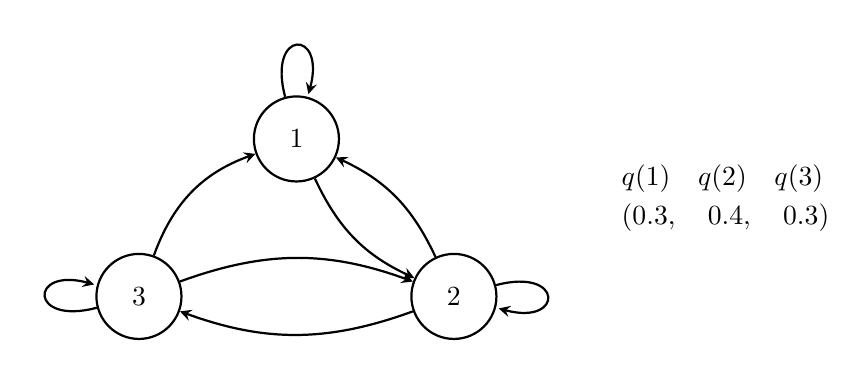
\begin{tikzpicture}[->, >=stealth, node distance=2cm, thick]

% Nodos de estados en disposición triangular
\node[circle, draw, inner sep=8pt] (s1) at (0,2) {1};
\node[circle, draw, inner sep=8pt] (s2) at (2,0) {2};
\node[circle, draw, inner sep=8pt] (s3) at (-2,0) {3};

% Bucles (self-loops)
\path (s1) edge[loop above] (s1);
\path (s2) edge[loop right] (s2);
\path (s3) edge[loop left] (s3);

% Transiciones entre estados
\path (s1) edge[bend right=20] (s2);
\path (s2) edge[bend right=20] (s1);
\path (s2) edge[bend left=20] (s3);
\path (s3) edge[bend left=20] (s2);
% Agregar 3 -> 1
\path (s3) edge[bend left=25] (s1);

% Distribución inicial
\node[right] at (4,1.5) {$q(1) \quad q(2) \quad q(3)$};
\node[right] at (4,1) {$(0.3, \quad 0.4, \quad 0.3)$};

\end{tikzpicture}
\end{center}

\definicion{La medida $q(i) = P(X_0 = i)$ definida para todo $i \in S$ se conoce como \textbf{distribución inicial} de la cadena.}

\textbf{Propiedades}:

\begin{enumerate}
    \item $0 \leq q(i)$ para $i \in S$.
    \item $\sum_{i \in S} q(i) = 1$.
    \item $P(X_n = j)$:

    \begin{align*}
    P(X_n = j) &= \sum_{i \in S} P(X_n = j, X_0 = i) \\
    &= \sum_{i \in S} P(X_n = j, X_0 = i) \cdot \frac{P(X_0 = i)}{P(X_0 = i)} \\
    &= \sum_{i \in S} P(X_n = j \mid X_0 = i) \cdot P(X_0 = i) \\
    &= \sum_{i \in S} P^n(i,j) \cdot q(i)
    \end{align*}
\end{enumerate}

\textbf{Nota:} $P(X_n = j)$ es la multiplicación del vector $q$ con la columna $j$ de la matriz $P^{(n)}$.

\textbf{Problema}: Considere una máquina que al inicio del día está funcionando o está dañada.

\begin{itemize}
    \item Estado 0 = Dañada
    \item Estado 1 = En buen estado
\end{itemize}

Suponga que el 20\% de los días la máquina amanece dañada, y tiene una matriz de transición:

\begin{equation*}
P = \begin{pmatrix}
0.3 & 0.7 \\
0.4 & 0.6
\end{pmatrix}
\end{equation*}

Determinar:
\begin{enumerate}
    \item $P(X_2 = 0, X_1 = 1, X_0 = 0) = q(0) P(0,1) P(1,0)$
    \item $P(X_1 = 0)$
    \item $P(X_2 = 0)$
\end{enumerate}

\textbf{Solución}:

$q = (0.2, 0.8)$ donde $q(0) = P(X_0 = 0)$

\begin{center}
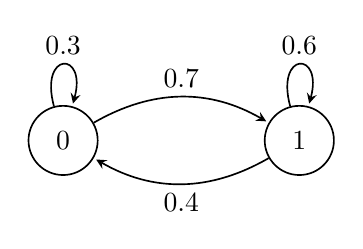
\begin{tikzpicture}[->,>=stealth,shorten >=1pt,auto,node distance=3cm,semithick]
\tikzstyle{every state}=[fill=white,draw=black,text=black,minimum size=25pt]
\node[state] (A) {$0$};
\node[state] (B) [right of=A] {$1$};
\path
(A) edge[loop above] node{$0.3$} (A)
(A) edge[bend left] node{$0.7$} (B)
(B) edge[bend left] node{$0.4$} (A)
(B) edge[loop above] node{$0.6$} (B);
\end{tikzpicture}
\end{center}

\textbf{1)} $P(X_2 = 0, X_1 = 1, X_0 = 0)$:

Por la propiedad de Markov:
\begin{align*}
P(X_2 = 0, X_1 = 1, X_0 = 0) &= P(X_2 = 0 \mid X_1 = 1) P(X_1 = 1 \mid X_0 = 0) P(X_0 = 0) \\
&= P(1,0) \times P(0,1) \times q(0) \\
&= 0.4 \times 0.7 \times 0.2 = 0.056
\end{align*}

\textbf{2)} $P(X_1 = 0) = q(0) P(0,0) + q(1) P(1,0) = 0.2 \times 0.3 + 0.8 \times 0.4 = 0.38$

\textbf{3)} $P(X_2 = 0) = P(X_2 = 0, X_1 = 0) + P(X_2 = 0, X_1 = 1)$

\begin{align*}
&= P(X_2 = 0 \mid X_1 = 0) P(X_1 = 0) + P(X_2 = 0 \mid X_1 = 1) P(X_1 = 1) \\
&= P(0,0) P(X_1 = 0) + P(1,0) P(X_1 = 1) \\
&= 0.3 \times 0.38 + 0.4 (1 - P(X_1 = 0)) \\
&= 0.3 \times 0.38 + 0.4 \times 0.62 = 0.36
\end{align*}

\section*{Clasificación de estados de una cadena de Markov}

\definicion{Un estado $j$ es \textbf{accesible} desde un estado $i$ si existe $n \geq 0$ tal que
\begin{equation*}
P_{ij}^{(n)} > 0
\end{equation*}
y lo denotamos por $i \to j$.}

\definicion{Si $i \to j$ y $j \to i$ entonces se dice que $i$ y $j$ se comunican, y denotamos por $i \leftrightarrow j$.

\begin{itemize}
    \item \textbf{Reflexiva:} Para todo $i \in S$, $i \to i$. $P_{ii}^{(0)} = 1 > 0$.
    \item \textbf{Simétrica:} Si $i \leftrightarrow j$ entonces $j \leftrightarrow i$.
    \item \textbf{Transitiva:} Si $i \leftrightarrow k$ y $k \leftrightarrow j$ entonces $i \leftrightarrow j$.
\end{itemize}

}

\textbf{Observación}: La relación $\leftrightarrow$ es de equivalencia.

\textbf{Demostración:} $i \leftrightarrow k$; existe $n \geq 0$ tal que $P_{ik}^{(n)} > 0$

$k \leftrightarrow j$; existe $m \geq 0$ tal que $P_{kj}^{(m)} > 0$.

\begin{equation*}
P_{ij}^{(n+m)} = \sum_{l \in S} P_{il}^{(n)} P_{lj}^{(m)} \geq P_{ik}^{(n)} P_{kj}^{(m)} > 0.
\end{equation*}


Las clases de equivalencia en una cadena de Markov (o en cualquier relación de equivalencia en matemáticas) forman una partición del espacio de estados. Eso significa:

\begin{itemize}
    \item Cada estado pertenece a una sola clase.
    \item Las clases son disjuntas entre sí.
    \item La unión de todas las clases cubre todos los estados.
\end{itemize}


\textbf{Problema}: Determine las clases de Equivalencia

\begin{equation*}
P = \begin{pmatrix}
1/2 & 1/2 & 0 \\
0 & 1/2 & 1/2 \\
0 & 1/3 & 2/3
\end{pmatrix}
\end{equation*}

\begin{center}
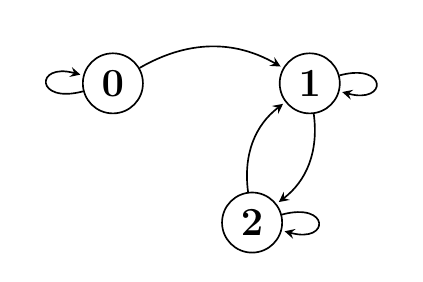
\begin{tikzpicture}[->,>=stealth,shorten >=1pt,auto,node distance=2.5cm,
    semithick,state/.style={circle,draw,font=\bfseries\Large}]

  \node[state] (0)                    {0};
  \node[state] (1) [right of=0]       {1};
  \node[state] (2) [below right of=0] {2};

  \path (0) edge [loop left] node {} (0)
            edge [bend left] node {} (1);
  \path (1) edge [loop right] node {} (1)
            edge [bend left] node {} (2);
  \path (2) edge [loop right] node {} (2)
            edge [bend left] node {} (1);
\end{tikzpicture}
\end{center}


\begin{align*}
1 &\leftrightarrow 2 \\
0 &\leftrightarrow 0 \\
C_A &= \{1, 2\} \\
C_B &= \{0\}
\end{align*}

En resumen:

\begin{itemize}
    \item Espacio de estados: $S = \{0, 1, 2\}$
    \item Clases de equivalencia encontradas: $C_A = \{1, 2\}$ y $C_B = \{0\}$
    \item Son disjuntas: $\{1, 2\} \cap \{0\} = \emptyset$
    \item Cubren todo el espacio de estados: $\{1, 2\} \cup \{0\} = \{0, 1, 2\}$
\end{itemize}

\definicion{Se dice que una cadena de Markov es irreducible si existe una única clase, es decir, todos los estados se comunican entre sí.}

\subsection*{Estados transitorios y recurrentes.}

\definicion{Sea
\begin{equation*}
f_{ii}^{(n)} = P(X_n=i, X_{n-1} \neq i, \dots, X_1 \neq i | X_0=i)
\end{equation*}
La probabilidad de primer retorno al estado $i$ en $n$ pasos, dado que se inició en $i$, se define como:
\begin{equation*}
f_i = \sum_{n=1}^{\infty} f_{ii}^{(n)} \quad \text{probabilidad de que regrese al estado i eventualmente}
\end{equation*}

Diremos que el estado $i$ es:
\begin{itemize}
    \item \textbf{Recurrente:} si $f_i = 1 \iff 1 - f_i = 0$
    \item \textbf{Transitorio:} si $f_i < 1 \iff 1 - f_i > 0$
\end{itemize}}

\textbf{Ejemplo}: Sea la cadena de Markov con matriz de transición:

\begin{equation*}
P = \begin{pmatrix}
1/2 & 1/2 & 0 \\
0 & 1/2 & 1/2 \\
0 & 1/3 & 2/3
\end{pmatrix}
\end{equation*}

\begin{center}
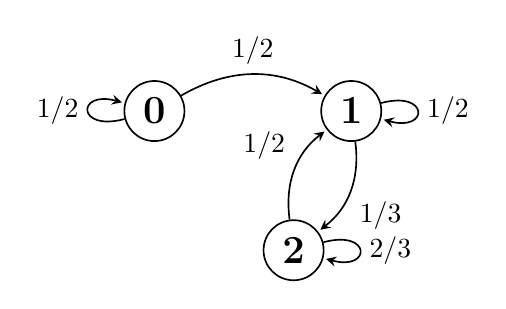
\begin{tikzpicture}[->,>=stealth,shorten >=1pt,auto,node distance=2.5cm,
    semithick,state/.style={circle,draw,font=\bfseries\Large}]

  \node[state] (0)                    {0};
  \node[state] (1) [right of=0]       {1};
  \node[state] (2) [below right of=0] {2};

  \path (0) edge [loop left] node {$1/2$} (0)
            edge [bend left] node {$1/2$} (1);
  \path (1) edge [loop right] node {$1/2$} (1)
            edge [bend left] node {$1/3$} (2);
  \path (2) edge [loop right] node {$2/3$} (2)
            edge [bend left] node {$1/2$} (1);
\end{tikzpicture}
\end{center}

Se procede a calcular $f_0$:

\begin{align*}
f_{00}^{(1)} &= P(X_1=0 \mid X_0=0) = 1/2 \\
f_{00}^{(2)} &= P(X_2=0, X_1 \neq 0 \mid X_0=0) = P(0,1) \cdot P(1,0) = \frac{1}{2} \cdot 0 = 0 \\
f_{00}^{(3)} &= P(X_3=0, X_2 \neq 0, X_1 \neq 0 \mid X_0=0) = P(0,1) \cdot P(1,2) \cdot P(2,0) = \frac{1}{2} \cdot \frac{1}{2} \cdot 0 = 0
\end{align*}

Para $n \geq 4$, observamos que $f_{00}^{(n)} = 0$ porque desde el estado 0 no podemos regresar sin pasar por el estado 1, y desde el estado 1 no podemos regresar al estado 0 (ya que $P(1,0) = 0$). Por lo tanto:
\begin{equation*}
f_{00}^{(n)} = \begin{cases}
1/2 & \text{si } n = 1 \\
0 & \text{si } n \geq 2
\end{cases}
\end{equation*}

\begin{equation*}
f_0 = \sum_{n=1}^{\infty} f_{00}^{(n)} = \frac{1}{2} + 0 + 0 + \cdots = \frac{1}{2} < 1
\end{equation*}

El estado $0$ es \textbf{transitorio}.

Se procede a calcular $f_1$.


\begin{align*}
f_{11}^{(1)} &= P(X_1=1 \mid X_0=1) = 1/2 \\
f_{11}^{(2)} &= P(X_2=1, X_1 \neq 1 \mid X_0=1) = P(1,2) \cdot P(2,1) = \frac{1}{2} \cdot \frac{1}{3} = \frac{1}{6} \\
f_{11}^{(3)} &= P(X_3=1, X_2 \neq 1, X_1 \neq 1 \mid X_0=1) = P(1,2) \cdot P(2,2) \cdot P(2,1) = \frac{1}{2} \cdot \frac{2}{3} \cdot \frac{1}{3} = \frac{1}{9}
\end{align*}

\begin{align*}
f_{11}^{(4)} &= P(X_4=1, X_3 \neq 1, X_2 \neq 1, X_1 \neq 1 \mid X_0=1) \\
&= P(1,2) \cdot P(2,2) \cdot P(2,2) \cdot P(2,1) \\
&= \frac{1}{2} \cdot \frac{2}{3} \cdot \frac{2}{3} \cdot \frac{1}{3} = \frac{2}{27}
\end{align*}

En general, para $n \geq 2$:
\begin{equation*}
f_{11}^{(n)} = P(1,2) \cdot [P(2,2)]^{n-2} \cdot P(2,1) = \frac{1}{2} \cdot \left(\frac{2}{3}\right)^{n-2} \cdot \frac{1}{3} = \frac{1}{6} \left(\frac{2}{3}\right)^{n-2}
\end{equation*}

Por lo tanto:
\begin{equation*}
f_{11}^{(n)} = \begin{cases}
1/2 & \text{si } n = 1 \\
\frac{1}{6} \left(\frac{2}{3}\right)^{n-2} & \text{si } n \geq 2
\end{cases}
\end{equation*}

\begin{align*}
f_1 &= \sum_{n=1}^{\infty} f_{11}^{(n)} \\
&= 1/2 + \sum_{n=2}^{\infty} 1/6 (2/3)^{n-2} \\
&= 1/2 + 1/6 \sum_{k=0}^{\infty} (2/3)^k \\
&= 1/2 + 1/6 \left(\frac{1}{1 - 2/3}\right) \\
&= 1/2 + 1/6 \cdot 3 \\
&= 1/2 + 1/2 = 1
\end{align*}

Por lo tanto, el estado $1$ es \textbf{recurrente}.

Se procede a calcular $f_2$.

\begin{align*}
f_{22}^{(1)} &= P(X_1=2 \mid X_0=2) = 2/3 \\
f_{22}^{(2)} &= P(X_2=2, X_1 \neq 2 \mid X_0=2) = P(2,1) \cdot P(1,2) = \frac{1}{3} \cdot \frac{1}{2} = \frac{1}{6} \\
f_{22}^{(3)} &= P(X_3=2, X_2 \neq 2, X_1 \neq 2 \mid X_0=2) = P(2,1) \cdot P(1,1) \cdot P(1,2) = \frac{1}{3} \cdot \frac{1}{2} \cdot \frac{1}{2} = \frac{1}{12}
\end{align*}

En general, para $n \geq 2$:
\begin{equation*}
f_{22}^{(n)} = P(2,1) \cdot [P(1,1)]^{n-2} \cdot P(1,2) = \frac{1}{3} \cdot \left(\frac{1}{2}\right)^{n-2} \cdot \frac{1}{2} = \frac{1}{6} \left(\frac{1}{2}\right)^{n-2}
\end{equation*}

Por lo tanto:
\begin{equation*}
f_{22}^{(n)} = \begin{cases}
2/3 & \text{si } n = 1 \\
\frac{1}{6} \left(\frac{1}{2}\right)^{n-2} & \text{si } n \geq 2
\end{cases}
\end{equation*}

\begin{align*}
f_2 &= \sum_{n=1}^{\infty} f_{22}^{(n)} \\
&= \frac{2}{3} + \sum_{n=2}^{\infty} \frac{1}{6} \left(\frac{1}{2}\right)^{n-2} \\
&= \frac{2}{3} + \frac{1}{6} \sum_{k=0}^{\infty} \left(\frac{1}{2}\right)^k \\
&= \frac{2}{3} + \frac{1}{6} \cdot \frac{1}{1 - 1/2} \\
&= \frac{2}{3} + \frac{1}{6} \cdot 2 \\
&= \frac{2}{3} + \frac{1}{3} = 1
\end{align*}

El estado $2$ es \textbf{recurrente}.


\begin{mdframed}[
    backgroundcolor=blue!10,
    linecolor=blue,
    linewidth=1pt,
    roundcorner=5pt,
    innertopmargin=10pt,
    innerbottommargin=10pt,
    innerleftmargin=10pt,
    innerrightmargin=10pt
]
Recordemos que: $ \forall i \in S$

\begin{equation}
f_{ii}^{(n)} = P(X_n=i, X_{n-1} \neq i, \dots, X_1 \neq i \mid X_0=i)
\end{equation}

\begin{equation}
f_i = \sum_{n=1}^{\infty} f_{ii}^{(n)}
\end{equation}

\rule{0.4\textwidth}{0.4pt}

$f_i < 1$ - $i$ transitorio

$f_i = 1$ - $i$ recurrente
\end{mdframed}


\teorema{Para una cadena de Markov con matriz de transición $P = (P_{ij})$:
\begin{itemize}
    \item $\sum_{n=0}^{\infty} P_{ii}^{(n)} = \infty$ si, y solo si el estado $i$ es recurrente
    \item $\sum_{n=0}^{\infty} P_{ii}^{(n)} < \infty$ si, y solo si el estado $i$ es transitorio
\end{itemize}}

\textbf{Demostración:} Tarea.

\textbf{Propiedad}: Sean $j$ y $k$ estados de una cadena de Markov entonces:

\begin{enumerate}
    \item Si $j$ es recurrente y $j \leftrightarrow k$ entonces $k$ es recurrente
    \item Si $j$ es transitorio y $j \leftrightarrow k$ entonces $k$ es transitorio
\end{enumerate}

\textbf{Demostración}: Sea $j$ recurrente y $j \leftrightarrow k$.

\begin{itemize}
    \item $j$ recurrente $\leftrightarrow \sum_{t=0}^{\infty} P_{jj}^{(t)} = \infty$
    \item $j \leftrightarrow k \leftrightarrow$ existen $m, n$ tales que $P_{jk}^{(n)} > 0$ y $P_{kj}^{(m)} > 0$
\end{itemize}

\begin{equation*}
P_{kk}^{n+m+t} \geq P_{kj}^{(m)} P_{jj}^{(t)} P_{jk}^{(n)}
\end{equation*}

\begin{equation*}
\sum_{t=0}^{\infty} P_{kk}^{n+m+t} \geq P_{kj}^{(m)} P_{jk}^{(n)} \sum_{t=0}^{\infty} P_{jj}^{(t)} = \infty
\end{equation*}

Por teorema presentado anteriormente $k$ es recurrente.

\textbf{Nota}: La demostración del caso transitorio es análoga.

\textbf{Propiedad}: Sea $X_n$ una cadena de Markov y $j$ uno de sus estados. El estado $j$ es recurrente, si y solo si el número esperado de visitas al estado $j$ es infinito, comenzando en $j$.

\textbf{Demostración}: Iniciamos por:

\begin{equation*}
E(I_n) = P(X_n = j)
\end{equation*}

Sea $I_n$ la variable aleatoria que indica cuantas veces la cadena pasa por el estado $j$:

\begin{equation*}
I_n = \begin{cases}
1 & \text{si } X_n=j \\
0 & \text{si } X_n \neq j
\end{cases}
\end{equation*}

$P(X_1=j \mid X_0=j)$

$P(X_2=j \mid X_0=j)$

\begin{center}
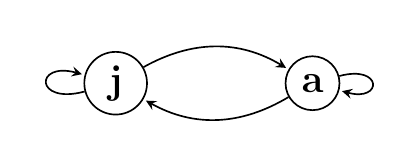
\begin{tikzpicture}[->,>=stealth,shorten >=1pt,auto,node distance=2.5cm,
    semithick,state/.style={circle,draw,font=\bfseries\Large}]

  \node[state] (j)                    {j};
  \node[state] (a) [right of=j]       {a};

  \path (j) edge [loop left] node {} (j)
            edge [bend left] node {} (a);
  \path (a) edge [loop right] node {} (a)
            edge [bend left] node {} (j);
\end{tikzpicture}
\end{center}

$\sum_{n=0}^{\infty} I_n :=$ número de visitas al estado $j$

\begin{align*}
E\left(\sum_{n=0}^{\infty} I_n \mid X_0=j\right) &= \sum_{n=0}^{\infty} E(I_n \mid X_0=j) \\
&= \sum_{n=0}^{\infty} P(X_n=j \mid X_0=j) \\
&= \sum_{n=0}^{\infty} P_{jj}^{(n)} = \infty
\end{align*}

\begin{center}
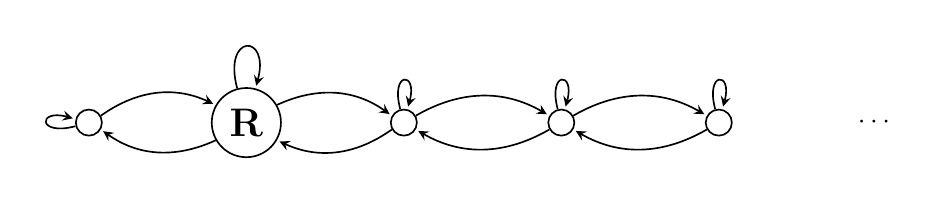
\begin{tikzpicture}[->,>=stealth,shorten >=1pt,auto,node distance=2cm,
    semithick,state/.style={circle,draw,font=\bfseries\Large}]

  \node[state] (1)                    {};
  \node[state] (2) [right of=1]       {R};
  \node[state] (3) [right of=2]       {};
  \node[state] (4) [right of=3]       {};
  \node[state] (5) [right of=4]       {};

  \path (1) edge [loop left] node {} (1)
            edge [bend left] node {} (2);
  \path (2) edge [loop above] node {} (2)
            edge [bend left] node {} (1)
            edge [bend left] node {} (3);
  \path (3) edge [loop above] node {} (3)
            edge [bend left] node {} (2)
            edge [bend left] node {} (4);
  \path (4) edge [loop above] node {} (4)
            edge [bend left] node {} (3)
            edge [bend left] node {} (5);
  \path (5) edge [loop above] node {} (5)
            edge [bend left] node {} (4);

  \node[right of=5] {$\cdots$};
\end{tikzpicture}
\end{center}

\definicion{Sea
\begin{equation*}
\tau_i = \min\{n \geq 1: X_n=i\}
\end{equation*}
el tiempo de retorno al estado $i$.

\begin{equation*}
E(\tau_i \mid X_0=i)
\end{equation*}
es el tiempo esperado de retorno al estado $i$.

\begin{equation*}
m_i = E(\tau_i \mid X_0=i) = \sum_{n=1}^{\infty} n \cdot f_{ii}^{(n)}
\end{equation*}}

\definicion{Se dice que un estado recurrente es:
\begin{enumerate}
    \item recurrente positivo si $m_i < \infty$.
    \item recurrente nulo si $m_i = \infty$.
\end{enumerate}}

\textbf{Observación}: Si el espacio de estados $S$ es finito todo estado recurrente es recurrente positivo. Si además $j$ es recurrente positivo (nulo) y $j \leftrightarrow k$ entonces $k$ es recurrente positivo (nulo).

\textbf{Ejemplo}:

\begin{center}
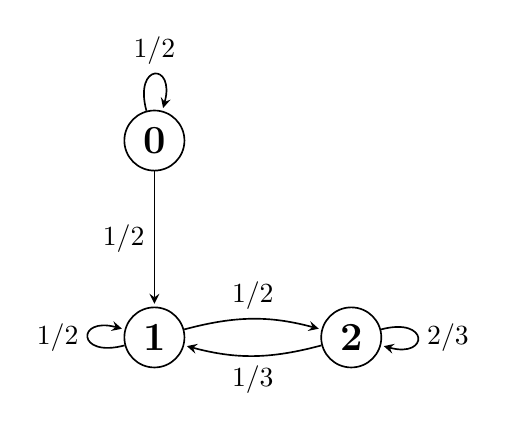
\begin{tikzpicture}[->,>=stealth,shorten >=1pt,auto,node distance=2.5cm,
    semithick,state/.style={circle,draw,font=\bfseries\Large}]

  \node[state] (0)                    {0};
  \node[state] (1) [below of=0]       {1};
  \node[state] (2) [right of=1]       {2};

  \path (0) edge [loop above] node {$1/2$} (0)
            edge [left] node {$1/2$} (1);
  \path (1) edge [loop left] node {$1/2$} (1)
            edge [bend left=15,above] node {$1/2$} (2);
  \path (2) edge [loop right] node {$2/3$} (2)
            edge [bend left=15,below] node {$1/3$} (1);
\end{tikzpicture}
\end{center}

\begin{equation*}
f_{11}^{(n)} = \begin{cases}
1/2 & \text{Para } n=1 \\
1/6 (2/3)^{n-2} & \text{para } n>1
\end{cases}
\end{equation*}

\begin{align*}
m_1 &= \sum_{n=1}^{\infty} n f_{11}^{(n)} = \frac{1}{2} + \sum_{n=2}^{\infty} n \frac{1}{6} \left(\frac{2}{3}\right)^{n-3} \\
&= \frac{1}{2} + \frac{1}{6} \sum_{k=0}^{\infty} (k+2) \left(\frac{2}{3}\right)^k \\
&= \frac{1}{2} + \frac{1}{6} \left(\sum_{k=0}^{\infty} k \left(\frac{2}{3}\right)^k + 2 \sum_{k=0}^{\infty} \left(\frac{2}{3}\right)^k\right) \\
&= \frac{1}{2} + \frac{1}{6} \left(\sum_{k=0}^{\infty} k \left(\frac{2}{3}\right)^k + 2 \left(\frac{1}{1 - 2/3}\right)\right) \\
&= \frac{1}{2} + \frac{1}{6} \left(\sum_{k=0}^{\infty} k \left(\frac{2}{3}\right)^k + 6\right) \\
&= \frac{1}{2} + \frac{1}{6} \sum_{k=0}^{\infty} k \left(\frac{2}{3}\right)^k + 1.
\end{align*}

\begin{align*}
&= \frac{1}{2} + 1 + \frac{1}{6} \times \frac{3}{2} \sum_{k=1}^{\infty} k \left(\frac{2}{3}\right)^k \quad \text{geom}(2/3) \\
&= \frac{1}{2} + 1 + \frac{1}{6} \times \frac{3}{2} \left(\frac{2/3}{1 - 2/3}\right) \\
&= \frac{1}{2} + 1 + \frac{1}{6} \times 3 \times \frac{2}{3} = \frac{1}{2} + 1 + \frac{1}{3} = \frac{11}{6}
\end{align*}

El 1 es recurrente positivo; pues $m_1 = \frac{11}{6} < \infty$.

Y como $1 \leftrightarrow 2$ entonces 2 es recurrente positivo.

\textbf{Ejemplo}: Consideremos la siguiente cadena de Markov.

\begin{equation*}
P_{ij} = \begin{cases}
1 & \text{si } i = 0, j = 1 \\
\frac{i}{i+1} & \text{si } i \geq 1, j = i+1 \\
\frac{1}{i+1} & \text{si } i \geq 1, j = 0 \\
0 & \text{e.o.c.}
\end{cases}
\end{equation*}

\begin{center}
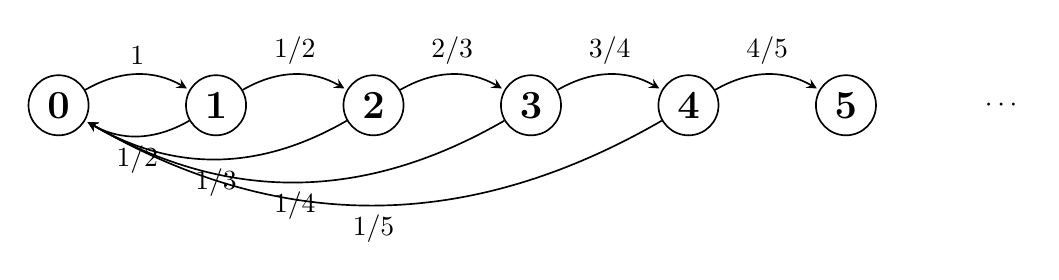
\begin{tikzpicture}[->,>=stealth,shorten >=1pt,auto,node distance=2cm,
    semithick,state/.style={circle,draw,font=\bfseries\Large}]

  \node[state] (0)                    {0};
  \node[state] (1) [right of=0]       {1};
  \node[state] (2) [right of=1]       {2};
  \node[state] (3) [right of=2]       {3};
  \node[state] (4) [right of=3]       {4};
  \node[state] (5) [right of=4]       {5};

  \path (0) edge [bend left,above] node {$1$} (1);
  \path (1) edge [bend left,below] node {$1/2$} (0)
            edge [bend left,above] node {$1/2$} (2);
  \path (2) edge [bend left,below] node {$1/3$} (0)
            edge [bend left,above] node {$2/3$} (3);
  \path (3) edge [bend left,below] node {$1/4$} (0)
            edge [bend left,above] node {$3/4$} (4);
  \path (4) edge [bend left,below] node {$1/5$} (0)
            edge [bend left,above] node {$4/5$} (5);

  \node[right of=5] {$\cdots$};
\end{tikzpicture}
\end{center}

¿D es recurrente? y ¿0 es positivo o nulo?

C

\begin{align*}
f_{00}^{(1)} &= P(X_1=0 \mid X_0=0) = 0 \\
f_{00}^{(2)} &= P(X_2=0, X_1 \neq 0 \mid X_0=0) = P(0,1) P(1,0) = 1/2 \\
f_{00}^{(3)} &= P(X_3=0, X_2 \neq 0, X_1 \neq 0 \mid X_0=0) = P(0,1) P(1,2) P(2,0) = 1 \times 1/2 \times 1/3
\end{align*}

\begin{align*}
f_{00}^{(4)} &= P(X_4=0, X_3 \neq 0, X_2 \neq 0, X_1 \neq 0 \mid X_0=0) \\
&= P(0,1) P(1,2) P(2,3) P(3,0) \\
&= 1 \times 1/2 \times 2/3 \times 1/4 = 1/3 \times 1/4
\end{align*}

\begin{align*}
f_{00}^{(5)} &= P(X_5=0, X_4 \neq 0, X_3 \neq 0, X_2 \neq 0, X_1 \neq 0 \mid X_0=0) \\
&= P(0,1) P(1,2) P(2,3) P(3,4) P(4,0) \\
&= 1 \times 1/2 \times 2/3 \times 3/4 \times 1/5 = 1/4 \times 1/5
\end{align*}


\begin{equation}
f_{00}^{(n)} = \frac{1}{n} \times \frac{1}{n-1} \quad \text{para } n \geq 2
\end{equation}

¿$f_0 = 1$?

\begin{align*}
f_0 &= \sum_{n=1}^{\infty} f_{00}^{(n)} \\
&= \sum_{n=2}^{\infty} \frac{1}{n} \times \frac{1}{n-1} \\
&= \sum_{n=2}^{\infty} \left(\frac{1}{n-1} - \frac{1}{n}\right)
\end{align*}

Serie telescópica:
\begin{equation}
1/1 - 1/2 + 1/2 - 1/3 + 1/3 - 1/4 + 1/4 - 1/5 + \cdots + 1/(m-1) - 1/m
\end{equation}

\begin{align*}
&= 1 - 1/m \\
f_0 &= \lim_{m \to \infty} \left(1 - \frac{1}{m}\right) = 1
\end{align*}

\textbf{Ejemplo:} Consideremos la siguiente cadena de Markov.

\begin{equation*}
P_{ij} = \begin{cases}
1 & \text{si } i=0, j=1 \\
\frac{i}{i+1} & \text{para } i \geq 1, j=i+1 \\
\frac{1}{i+1} & \text{para } i \geq 1, j=0 \\
0 & \text{e.o.c.}
\end{cases}
\end{equation*}

\begin{align*}
m_0 &= \sum_{n=1}^{\infty} n f_{00}^{(n)} \\
&= \sum_{n=2}^{\infty} n \frac{1}{n} \frac{1}{n-1} \\
&= \sum_{n=2}^{\infty} \frac{1}{n-1} \\
&= \infty
\end{align*}

El estado 0 es recurrente nulo y como $j \leftrightarrow 0$; $j \in S$ entonces todos los estados son recurrentes nulos.

\begin{center}
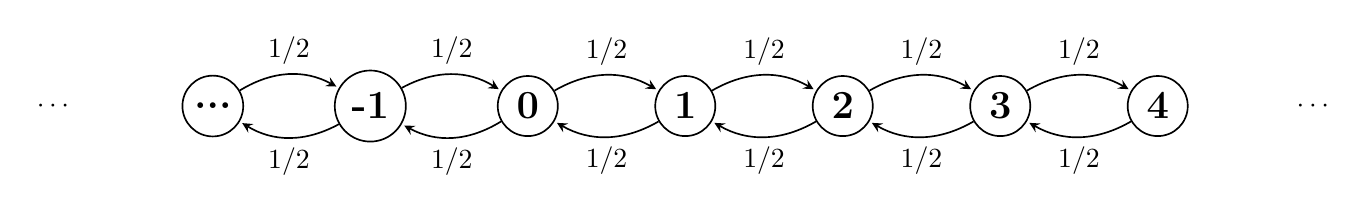
\begin{tikzpicture}[->,>=stealth,shorten >=1pt,auto,node distance=2cm,
    semithick,state/.style={circle,draw,font=\bfseries\Large}]
  \node[state] (-2)                   {...};
  \node[left of=-2] {$\cdots$};
  \node[state] (-1) [right of=-2]     {-1};
  \node[state] (0) [right of=-1]      {0};
  \node[state] (1) [right of=0]       {1};
  \node[state] (2) [right of=1]       {2};
  \node[state] (3) [right of=2]       {3};
  \node[state] (4) [right of=3]       {4};
  \node[right of=4] {$\cdots$};

  \path (-2) edge [bend left,above] node {$1/2$} (-1);
  \path (-1) edge [bend left,above] node {$1/2$} (0)
            edge [bend left,below] node {$1/2$} (-2);
  \path (0) edge [bend left,below] node {$1/2$} (-1)
            edge [bend left,above] node {$1/2$} (1);
  \path (1) edge [bend left,below] node {$1/2$} (0)
            edge [bend left,above] node {$1/2$} (2);
  \path (2) edge [bend left,below] node {$1/2$} (1)
            edge [bend left,above] node {$1/2$} (3);
  \path (3) edge [bend left,below] node {$1/2$} (2)
            edge [bend left,above] node {$1/2$} (4);
  \path (4) edge [bend left,below] node {$1/2$} (3);
\end{tikzpicture}
\end{center}

$P^n(0,0) = \begin{cases}
> 0 & \text{si } n \text{ es par} \\
0 & \text{si } n \text{ es impar}
\end{cases}$

\section*{Periodicidad de la cadena}

\definicion{Se dice que el estado $i$ tiene periodo $d$ si
\begin{equation}
d = \text{mcd} \{n: P_{ii}^{(n)} > 0\}
\end{equation}

\begin{itemize}
    \item Si $d=1$ entonces el estado $i$ es aperiódico.
    \item Si $d>1$ entonces el estado $i$ es periódico.
\end{itemize}

Diremos que la cadena es aperiódica si todos sus estados son aperiódicos.

}

\textbf{Propiedades}:

\begin{enumerate}
    \item Si $i$ tiene periodo $d$ y $i \leftrightarrow j$ entonces $j$ tiene periodo $d$.
    \item Si $P_{ii} > 0$ entonces $i$ es aperiódico ($d=1$).
\end{enumerate}

\textbf{Ejemplo}: Considere

\begin{equation*}
P = \begin{pmatrix}
0.3 & 0 & 0 & 0 & 0.7 & 0 & 0 \\
0.1 & 0.2 & 0.3 & 0.4 & 0 & 0 & 0 \\
0 & 0.2 & 0 & 0.5 & 0.3 & 0 & 0 \\
0 & 0 & 0 & 0 & 0 & 0.5 & 0.5 \\
0.6 & 0 & 0 & 0 & 0.4 & 0 & 0 \\
0 & 0 & 0 & 0.4 & 0 & 0.2 & 0.4 \\
0 & 0 & 0 & 1 & 0 & 0 & 0
\end{pmatrix}
\end{equation*}


\begin{center}
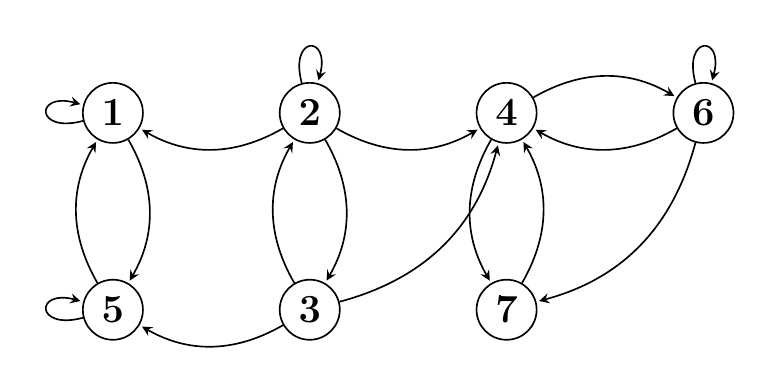
\begin{tikzpicture}[->,>=stealth,shorten >=1pt,auto,node distance=2.5cm,
    semithick,state/.style={circle,draw,font=\bfseries\Large}]

  \node[state] (1)                   {1};
  \node[state] (2) [right of=1]      {2};
  \node[state] (4) [right of=2]      {4};
  \node[state] (6) [right of=4]      {6};
  \node[state] (5) [below of=1]      {5};
  \node[state] (3) [below of=2]      {3};
  \node[state] (7) [below of=4]      {7};

  % Auto-loops (solo donde P_{ii} > 0)
  \path (1) edge [loop left] node {} (1);
  \path (2) edge [loop above] node {} (2);
  \path (5) edge [loop left] node {} (5);
  \path (6) edge [loop above] node {} (6);

  % Transitions according to matrix P
  % State 1: P(1,1)=0.3, P(1,5)=0.7
  \path (1) edge [bend left,above] node {} (5);
  
  % State 2: P(2,1)=0.1, P(2,2)=0.2, P(2,3)=0.3, P(2,4)=0.4
  \path (2) edge [bend left,above] node {} (1);
  \path (2) edge [bend left,above] node {} (3);
  \path (2) edge [bend right,above] node {} (4);
  
  % State 3: P(3,2)=0.2, P(3,4)=0.5, P(3,5)=0.3
  \path (3) edge [bend left,below] node {} (2);
  \path (3) edge [bend right,below] node {} (4);
  \path (3) edge [bend left,above] node {} (5);
  
  % State 4: P(4,6)=0.5, P(4,7)=0.5
  \path (4) edge [bend left,above] node {} (6);
  \path (4) edge [bend right,below] node {} (7);
  
  % State 5: P(5,1)=0.6, P(5,5)=0.4
  \path (5) edge [bend left,below] node {} (1);
  
  % State 6: P(6,4)=0.4, P(6,6)=0.2, P(6,7)=0.4
  \path (6) edge [bend left,below] node {} (4);
  \path (6) edge [bend left,above] node {} (7);
  
  % State 7: P(7,4)=1.0
  \path (7) edge [bend right,above] node {} (4);

\end{tikzpicture}
\end{center}

Las siguientes son las clases de equivalencia identificadas:

\begin{align*}
C_1 &= \{5, 1\} \\
C_2 &= \{3, 2\} \\
C_3 &= \{4, 6, 7\}
\end{align*}

Para cada estado $i$, calculamos $d_i = \text{mcd} \{n: P^n(i,i) > 0\}$:

\begin{align*}
d_1 &= \text{mcd} \{n: P^n(1,1) > 0\} = \text{mcd} \{1, 2, 3, \dots\} = 1 \\
d_5 &= 1 \\
d_3 &= \text{mcd} \{n: P^n(3,3) > 0\} = \text{mcd} \{2, 3, 4, 5, \dots\} = 1 \\
d_2 &= 1 \\
d_7 &= \text{mcd} \{n: P^n(7,7) > 0\} = \text{mcd} \{2, 3, 4, 5, 6, \dots\} = 1 \\
d_4 &= d_6 = 1
\end{align*}

\section*{Probabilidades Estacionarias}

\definicion{$\pi$ es una medida estacionaria si
\begin{equation}
\pi P = \pi
\end{equation}
donde $\pi P_j = P(X_n = j)$
}

\textbf{Ejemplo}: Considere la distribución inicial $\pi_0 = (0.2, 0.8)$ y la matriz de transición:

\begin{equation*}
P = \begin{pmatrix}
0.3 & 0.7 \\
0.1 & 0.9
\end{pmatrix}
\end{equation*}

Calculamos $P(X_1 = 0)$:

\begin{align*}
P(X_1 = 0) &= 0.3 \times 0.2 + 0.8 \times 0.1 \\
&= 0.06 + 0.08 \\
&= 0.14
\end{align*}

\textbf{Ejemplo}: Considere la matriz de transición:

\begin{equation*}
P = \begin{pmatrix}
0 & 3/4 & 1/4 \\
1/2 & 0 & 1/2 \\
1 & 0 & 0
\end{pmatrix}
\end{equation*}

¿Cuánto vale $\pi$?

La distribución estacionaria satisface $\pi P = \pi$:

\begin{equation*}
(\pi_1, \pi_2, \pi_3) \begin{pmatrix}
0 & 3/4 & 1/4 \\
1/2 & 0 & 1/2 \\
1 & 0 & 0
\end{pmatrix} = (\pi_1, \pi_2, \pi_3)
\end{equation*}

Esto nos da el sistema de ecuaciones:

\begin{align*}
\frac{1}{2} \pi_2 + \pi_3 &= \pi_1 \\
\frac{3}{4} \pi_1 &= \pi_2 \\
\frac{1}{4} \pi_1 + \frac{1}{2} \pi_2 &= \pi_3
\end{align*}

Con la condición de normalización:
\begin{equation}
\pi_1 + \pi_2 + \pi_3 = 1
\end{equation}

Resolviendo el sistema:

\begin{align*}
\pi_1 &= \frac{8}{19}, \quad \pi_2 = \frac{6}{19}, \quad \pi_3 = \frac{5}{19}
\end{align*}

Por lo tanto, $P(X_{m-1} = 1) = \frac{8}{19}$.

\textbf{Ejemplo}: Considere la matriz de transición:

\begin{equation*}
P = \begin{pmatrix}
1 & 0 & 0 \\
1/3 & 1/3 & 1/3 \\
0 & 0 & 1
\end{pmatrix}
\end{equation*}

Determina $\pi = (\pi_1, \pi_2, \pi_3)$.

\begin{center}
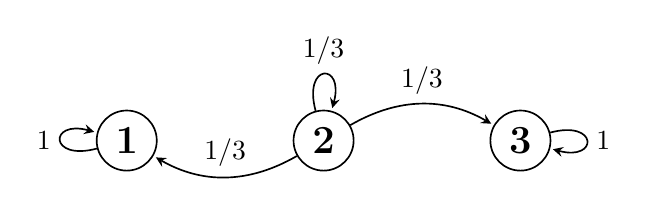
\begin{tikzpicture}[->,>=stealth,shorten >=1pt,auto,node distance=2.5cm,
    semithick,state/.style={circle,draw,font=\bfseries\Large}]

  \node[state] (1)                   {1};
  \node[state] (2) [right of=1]      {2};
  \node[state] (3) [right of=2]      {3};

  % Auto-loops
  \path (1) edge [loop left] node {$1$} (1);
  \path (2) edge [loop above] node {$1/3$} (2);
  \path (3) edge [loop right] node {$1$} (3);

  % Transitions
  \path (2) edge [bend left,above] node {$1/3$} (1);
  \path (2) edge [bend left,above] node {$1/3$} (3);

\end{tikzpicture}
\end{center}

La distribución estacionaria satisface $\pi P = \pi$:

\begin{equation*}
(\pi_1, \pi_2, \pi_3) \begin{pmatrix}
1 & 0 & 0 \\
1/3 & 1/3 & 1/3 \\
0 & 0 & 1
\end{pmatrix} = (\pi_1, \pi_2, \pi_3)
\end{equation*}

Esto nos da el sistema de ecuaciones:

\begin{align*}
\pi_1 + \frac{1}{3} \pi_2 &= \pi_1 \\
\frac{1}{3} \pi_2 &= \pi_2 \\
\frac{1}{3} \pi_2 + \pi_3 &= \pi_3
\end{align*}

De la segunda ecuación: $\frac{1}{3} \pi_2 = \pi_2 \Rightarrow \pi_2 = 0$

De la primera ecuación: $\pi_1 + \frac{1}{3} \pi_2 = \pi_1 \Rightarrow \pi_1 = \pi_1$ (siempre se cumple)

De la tercera ecuación: $\frac{1}{3} \pi_2 + \pi_3 = \pi_3 \Rightarrow \pi_3 = \pi_3$ (siempre se cumple)

Con la condición de normalización: $\pi_1 + \pi_2 + \pi_3 = 1$

Como $\pi_2 = 0$, tenemos: $\pi_1 + \pi_3 = 1$

Por lo tanto, $\pi = (\alpha, 0, 1-\alpha)$ donde $\alpha \in (0,1)$.

\textbf{Propiedad}: La cadena de Markov tiene una única medida estacionaria si es irreducible (recurrencia positiva).

\textbf{Propiedad}: Si $\pi$ es una medida estacionaria, entonces $X_n \sim \pi$. $P_{\pi}(X_n=j) = \pi(j)$.

\textbf{Demostración}:

\begin{itemize}
    \item $\pi P = \pi$
    \item $\pi P^2 = \pi P P = \pi P = \pi$
    \item Si $\pi P^n = \pi$ entonces:
    
    $\pi P^{n+1} = \pi P^n P = \pi P = \pi$
    
    Por lo tanto, $\pi P^n = \pi$ para todo $n \geq 1$.
\end{itemize}

Si $X_0 \sim \pi$ entonces $X_n \sim \pi$.
\begin{equation}
P(X_n=j) = \pi(j)
\end{equation}

\teorema{Si la cadena de Markov es irreducible y sus estados son recurrentes positivos, entonces la medida estacionaria $\pi$ existe y es única. Además:
\begin{equation*}
\pi_i = \frac{1}{m_i}, \quad i \in S
\end{equation*}
donde $m_i$ es el \textbf{tiempo medio de retorno} al estado $i$, es decir,
\begin{equation*}
m_i = E(\tau_i \mid X_0=i) = \sum_{n=1}^{\infty} n \cdot f_{ii}^{(n)}
\end{equation*}
(esperanza del tiempo hasta regresar a $i$ partiendo de $i$)
}

\begin{mdframed}[
    backgroundcolor=gray!10,
    linecolor=gray,
    linewidth=1pt,
    roundcorner=5pt,
    innertopmargin=10pt,
    innerbottommargin=10pt,
    innerleftmargin=10pt,
    innerrightmargin=10pt
]

\begin{itemize}
    \item $\lim_{n \to \infty} P^n(x,y) = \pi(y).$
    \item Si el estado $y$ es transitorio; $\sum_{n=1}^{\infty} P^n(x,y) < \infty$
    $\Rightarrow \lim_{n \to \infty} P^n(x,y) = 0.$
\end{itemize}

\begin{center}
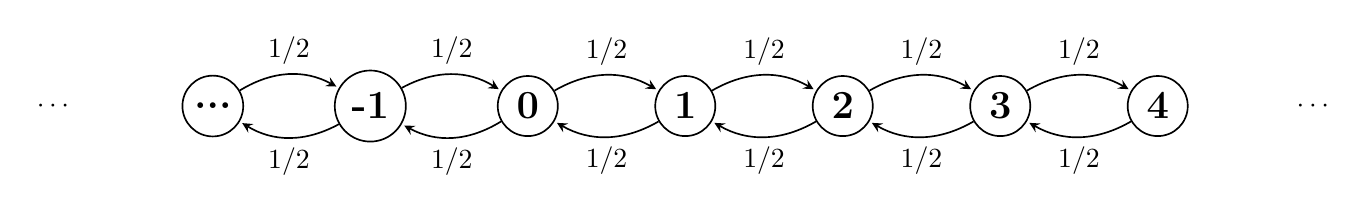
\begin{tikzpicture}[->,>=stealth,shorten >=1pt,auto,node distance=2cm,
    semithick,state/.style={circle,draw,font=\bfseries\Large}]
  \node[state] (-2)                   {...};
  \node[left of=-2] {$\cdots$};
  \node[state] (-1) [right of=-2]     {-1};
  \node[state] (0) [right of=-1]      {0};
  \node[state] (1) [right of=0]       {1};
  \node[state] (2) [right of=1]       {2};
  \node[state] (3) [right of=2]       {3};
  \node[state] (4) [right of=3]       {4};
  \node[right of=4] {$\cdots$};

  \path (-2) edge [bend left,above] node {$1/2$} (-1);
  \path (-1) edge [bend left,above] node {$1/2$} (0)
            edge [bend left,below] node {$1/2$} (-2);
  \path (0) edge [bend left,below] node {$1/2$} (-1)
            edge [bend left,above] node {$1/2$} (1);
  \path (1) edge [bend left,below] node {$1/2$} (0)
            edge [bend left,above] node {$1/2$} (2);
  \path (2) edge [bend left,below] node {$1/2$} (1)
            edge [bend left,above] node {$1/2$} (3);
  \path (3) edge [bend left,below] node {$1/2$} (2)
            edge [bend left,above] node {$1/2$} (4);
  \path (4) edge [bend left,below] node {$1/2$} (3);
\end{tikzpicture}
\end{center}

\begin{align*}
P^{2n+1}(0,0) &= 0 \\
P^{2n}(0,0) &> 0.
\end{align*}

$\lim_{n \to \infty} P^n(0,0)$ no existe!

$\lim_{n \to \infty} P^{dn}(0,0)$ sí existe.

\end{mdframed}

\teorema{Sea $X_n$ una cadena de Markov $\{X_n\}_{n \geq 0}$ cuyos estados son irreducibles; recurrentes positivos y aperiódicos. Entonces:
\begin{equation*}
\lim_{n \to \infty} P^n(x,y) = \pi(y)
\end{equation*}}

\textbf{Demostración}: Estudio personal.

\textbf{Observación}:

\begin{itemize}
    \item Si $S$ es finito todos los estados recurrentes son recurrentes positivos
    \item Si $S$ es finito entonces si es irreducible todos los estados son recurrentes positivos
\end{itemize}

\begin{mdframed}[
    backgroundcolor=blue!10,
    linecolor=blue,
    linewidth=1pt,
    roundcorner=5pt,
    innertopmargin=10pt,
    innerbottommargin=10pt,
    innerleftmargin=10pt,
    innerrightmargin=10pt
]

Si $X_1, X_2, \dots, X_n$ iid $f_i$, $E(|X|) < \infty$.

$\frac{1}{n} \sum_{i=1}^{n} X_i \xrightarrow{\text{C.S.}} E(X)$.

\end{mdframed}

\section*{Ley Fuerte de los Grandes Números}

Suponga que $\{X_n\}_{n \geq 1}$ cumplió con las condiciones del teorema anterior y sea $r(\cdot)$ una función tal que:
\begin{equation}
\sum_{x} |r(x)| \pi(x) < \infty
\end{equation}

entonces:
\begin{equation}
\frac{1}{n} \sum_{k=1}^{n} r(X_k) \xrightarrow{\text{C.S.}} E_{\pi}(r(X)) = \sum_{x} r(x) \pi(x)
\end{equation}

\textbf{Ejercicio}: Sea $X_n$ la cantidad de stock de un determinado producto en una tienda al final del día $n$ y $D_{n+1}$ la demanda del producto en el día $n+1$.

Cuando el stock al final del día es menor o igual a 1 unidad, ordenamos la cantidad necesaria para volver a tener 5 unidades.

\begin{equation*}
X_{n+1} = \begin{cases}
(X_n - D_{n+1})^+ & \text{si } X_n > 1 \\
(5 - D_{n+1})^+ & \text{si } X_n \leq 1
\end{cases}
\end{equation*}

Sea una cadena de Markov que:

\begin{center}
\begin{tabular}{|c|c|c|c|c|}
\hline
$k$ & 0 & 1 & 2 & 3 \\
\hline
$P(D_{n+1}=k)$ & 0.3 & 0.4 & 0.2 & 0.1 \\
\hline
\end{tabular}
\end{center}

\textbf{Problema 1}: Determina la matriz de transición.

\begin{align*}
P(0,0) &= 0 \\
P(0,1) &= 0 \\
P(0,2) &= P(D_{n+1}=3) = 0.1 \\
P(0,3) &= 0.2 \\
P(0,4) &= 0.4 \\
P(0,5) &= 0.3
\end{align*}

\begin{align*}
P(2,0) &= P(D_{n+1}=2 \text{ o } D_{n+1}=3) \\
&= P(D_{n+1}=2) + P(D_{n+1}=3)
\end{align*}

La matriz de transición completa es:

\begin{equation*}
P = \begin{pmatrix}
0 & 0 & 0.1 & 0.2 & 0.4 & 0.3 \\
0 & 0 & 0.1 & 0.2 & 0.4 & 0.3 \\
0.3 & 0.4 & 0.3 & 0 & 0 & 0 \\
0.1 & 0.2 & 0.4 & 0.3 & 0 & 0 \\
0 & 0.1 & 0.2 & 0.4 & 0.3 & 0 \\
0 & 0 & 0.1 & 0.2 & 0.4 & 0.3
\end{pmatrix}
\end{equation*}

\textbf{Problema 2}: Suponga que ganamos \$12 mil pesos por cada unidad vendida y tiene un costo de \$2 mil pesos almacenar. ¿Cuál es la ganancia a largo plazo por día?

Calculamos el período de la cadena:
\begin{equation*}
d = \text{mcd} \{n: P^n(0,0) > 0\}
\end{equation*}

\begin{align*}
P(0,0) &= 0 \\
P^2(0,0) &> 0 \\
P^3(0,0) &> 0
\end{align*}

\begin{equation*}
d = \text{mcd} \{2,3,4,5,\dots\} = 1
\end{equation*}

La distribución estacionaria satisface $\pi P = \pi$:
\begin{equation*}
\pi = \frac{1}{9740} (885, 1516, 2250, 2100, 1960, 1029)
\end{equation*}

Demanda esperada por día:
\begin{equation*}
E(D_{n+1}) = 0 \times 0.3 + 1 \times 0.4 + 2 \times 0.2 + 3 \times 0.1 = 1.1
\end{equation*}

¿Cuál es la pérdida por falta de stock a largo plazo?

Condición: $X_n = 2$ y $D_{n+1} = 3$

\begin{equation*}
\text{PFS} = \begin{cases}
1 & \text{si } X_n = 2; D_{n+1} = 3 \\
0 & \text{e.o.c.}
\end{cases}
\end{equation*}

\begin{align*}
E(\text{PFS}) &= 1 \times P(X_n = 2, D_{n+1} = 3) + 0 \times P(\text{otros casos}) \\
&= P(X_n = 2) \times P(D_{n+1} = 3) \\
&= \pi(2) \times 0.1 \\
&= \frac{2250}{9740} \times 0.1 = 0.0231
\end{align*}

Entrada por día:
\begin{equation*}
\text{Entrada} = 12\,\text{mil} \times (1.1 - 0.0231) = 12\,\text{mil} \times 1.0769 = 12.92\,\text{mil}
\end{equation*}

Salida por día (costo de almacenamiento):
\begin{align*}
r(X_k) &= 2\,\text{mil} \times X_k \\
E_{\pi}(r(X)) &= \sum_{x=0}^{5} r(x) \pi(x) \\
&= 2\,\text{mil} \times \sum_{x=0}^{5} x \cdot \pi(x) \\
&= \frac{2\,\text{mil}}{9740} \times (0 \times 885 + 1 \times 1516 + 2 \times 2250 + 3 \times 2100 + 4 \times 1960 + 5 \times 1029) \\
&= \frac{2\,\text{mil}}{9740} \times (0 + 1516 + 4500 + 6300 + 7840 + 5145) \\
&= \frac{2\,\text{mil}}{9740} \times 25301 \\
&= 5.20\,\text{mil}
\end{align*}

Ganancia diaria:
\begin{equation*}
\text{Ganancia} = 12.92 - 5.20 = 7.72\,\text{mil pesos}
\end{equation*}

\end{document}
